\documentclass[aspectratio=43, 10pt]{beamer}
\usepackage{tutorialSlide}
\usepackage{graphicx}               % Necessary to use \scalebox
\usepackage[absolute,overlay]{textpos}

\newcommand{\curl}{{\textbf{curl}}}


\mode<presentation> {
\usetheme{AnnArbor}
\usecolortheme{dolphin}

% Configure and Customize the theme
%\setbeamertemplate{theorems}[numbered]
\setbeamercolor{alerted text}{fg=red}
% Change color scheme for blocks
\setbeamercolor*{block title example}{fg = ao(english), bg= antiquewhite}
\setbeamercolor*{block title}{fg = pigment, bg= blue!5}
\setbeamercolor*{block title alerted}{fg = red, bg= red!5}
}

\makeatletter
\newcommand\mysphere{%
  \parbox[t]{8pt}{\raisebox{0.2pt}{\beamer@usesphere{item projected}{bigsphere}}}}
\makeatother




%***************************************************************************
%***************************************************************************
\begin{document}
\title{Inspecting NOMA from Information Theory}
\subtitle{The Art of Dealing with Interference}
\author{Weijia Zheng 
\thanks{I mainly take reference to: Chapter 5, "Multiple Access Techniques for 5G Wireless Networks and Beyond". Springer Publishing Company, Incorporated, by M. Vaezi, Z. Ding, and H. V. Poor. 2018.}
}

\institute[IE@CUHK] % Your institution as it will appear on the bottom of every slide, may be shorthand to save space
{
\textit{Department of Information Engineering} \\ % Your institution for the title page
\textit{The Chinese University of Hong Kong} \\
\medskip
wjzheng@link.cuhk.edu.hk % Your email address
}
\date{March 25, 2024}

\setcounter{framenumber}{-1}
\frame{\titlepage}
%***************************************************************************
%***************************************************************************




\begin{frame}
\frametitle{Overview} % Table of contents slide, comment this block out to remove it
\tableofcontents % Throughout your presentation, if you choose to use \section{} and \subsection{} commands, these will automatically be printed on this slide as an overview of your presentation
\end{frame}



\AtBeginSection[]
  {
     \begin{frame}<beamer>
     \frametitle{Overview}
     \tableofcontents[currentsection]
     \end{frame}
  }
  
  
\section{What is NOMA?}
  \begin{frame}[t]{Multiple Access, OMA and NOMA}
    Multiple access is of crucial importance of cellular communication systems. From 1G to 4G, different multiple access schemes are adopted. 
    \begin{block}{Multiple access methods used from 1G to 4G}
        \begin{itemize}
        \item Frequency division multiple access (FDMA, for 1G)
        \item Time division multiple access (TDMA, for 2G)
        \item Code division multiple access (CDMA, for 3G)
        \item Orthogonal frequency division multiple access (OFDMA, for 4G)
        \end{itemize}
    \end{block}
    One common idea: different users have orthogonal signals. Hence these above methods are usually considered as orthogonal multiple access (OMA). 
    \vfill
    
    \pause
    
    \begin{block}{The term "NOMA" is rather vague}
        Different people preceive the "non-orthogonality" in NOMA via different ways. 
        
        We present some of the definitions then. 
    \end{block}
  \end{frame}

   \begin{frame}[t]{3 Definitions of NOMA}
   \vspace{-1.3em}
        \begin{block}{Linear Transform in Decoding}
        This view requires OMA schemes to be: signals of different users can be separated into orthogonal subspaces using a linear transform. 
        
        And, any scheme does not meet such condition $\implies$ NOMA.
      \end{block}
      
      \pause
      \vspace{-0.7em}
      \begin{block}{Superposition coding \& Succesive interference cancellation (SC-SIC)}
          Many consider NOMA to be equivalent to schemes that use superposition coding at transmitter and successive interference cancellation at receiver (SC-SIC). Aka, SC-SIC $=$ NOMA. 
          % 
          
          \textcolor{red}{Given that SC-SIC achieves capacity of degraded downlink/broadcast channel, and the capacity of an uplink channel (MAC) can be regarded as doing SIC at the decoder.}
      \end{block}

      \pause 
       \vspace{-0.7em}
      \begin{block}{Information Theory Proving Mindset \& Technique}
        NOMA may refer to any technique allowing concurrent transmission is  over the same resources in time/frequency/code. This achieves a better rate region when compared to orthogonalizing of one or some of the resources. 
        \textcolor{red}{Under such viewpoint, SC-SIC $\subsetneq$ NOMA}
      \end{block}
  \end{frame}



  

\section{Why we need NOMA?}
  \begin{frame}[t]{Beyond orthogonal schemes}
    \vspace{-0.8em}
     We hope NOMA "to reap the benefits promised by information theory for the downlink and uplink transmission of wireless systems, modelled by the broadcast channel (BC) and multiple access channel (MAC)."

     \vfill
     
     Capacity regions of degraded BC and MAC have been established several decades ago (which we will see later), and concurrent non-orthogonal schemes are a must to achieve capacity.
    
    % \vfill
    \pause
    \begin{block}{Then... why from 1G to 4G we insisted on OMA?}
       This was mainly to avoid inter-user interference cancellation, which would have resulted in unacceptably complex receivers. 
       
       Some schemes of this type (avoiding interference cancellation), e.g., treat-interference-as-noise (TIN) are more practical. 
    \end{block}

    \pause
    \begin{block}{Okay, then... is it a good timing to use NOMA now?}
       \textcolor{purple}{If we are really going into an era of IoT, then yes.} 
       
       "Amazon alone has $>10^8$ devices already, and networks connects them operate in (congested) ISM bands (900MHz 2.4GHz)." Overhead of orthogonal schemes will be a nightmare, given such massive connectivity. 
    \end{block}  
  \end{frame}
    



\section{NOMA in single-cell: multiple access channel, and broadcast channel}
    \begin{frame}
        In the following, no matter for multiple access channel, broadcast channel or interference channel, we will mainly focus on Gaussian channels \textcolor{red}{without MIMO}. 

        \vfill
        But we do will mention some more general channel types for completeness. 

        \vfill 
        \begin{definition}[Gaussian capacity function]
        We define the Gaussian capacity function $\mathcal{C}(x), x\geq 0$ as
            $$\mathcal{C}(x) \coloneqq \frac{1}{2}\log(1+x).$$ 
        \end{definition}
                
        This gives the capacity of a point-to-point Gaussian channel, more precisely, if $$Y=gX + Z$$ with $Z\sim N(0,1)$ and $\mathbb{E} X^2 \leq P$. Then $\mathcal{C}(\frac{g^2 P}{1})= \mathcal{C}(\text{SNR}) = \frac{1}{2}\log(1+\text{SNR})$ gives you the channel capacity. 
    \end{frame}




    \begin{frame}[t]{Multiple Access Channel, Uplink \small ($K\geq2$ senders, 1 receiver)}
    \vspace{-1.1em}
    MAC is well-understood. Its general capacity is known. Most studies are done in 1970 $\sim$ 1985. 
    
    \vspace{-0.8em}
    \begin{columns}
    % Column 1
    \begin{column}{0.6\textwidth}
        \begin{block}{2-sender Gaussian MAC (single letter)}
        \small
            $$Y = g_1 X_1 + g_2 X_2 + Z,$$ 
            where $Z\sim N(0,1)$ is noise, $g_1, g_2$ are channel gains. $\mathbb{E}[X_i^2] \leq P$ is power constraint. 
        \end{block}
    \end{column}
    % Column 2    
    \begin{column}{0.4\textwidth}
        \begin{figure}
        \centering
            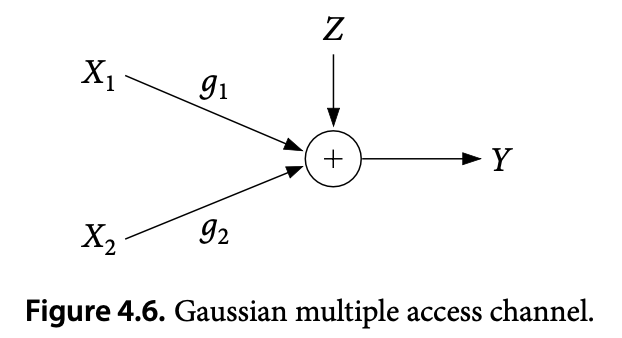
\includegraphics[width=0.9\textwidth]{figures/gaussian2txMAC.png}
            % \caption{A figure that is next to a certain explanation.}
        \end{figure}
    \end{column}
    \end{columns}

    \vspace{-0.8em}
    \begin{columns}

    % Column 1
    \begin{column}{0.57\textwidth}
    \small
        \begin{block}{K-sender GMAC Capacity (Cover, 1974)}
        The capacity region of the $K$-user Gaussian MAC is the set of all nonnegative $(R_1,...,R_K)$ such that $$\sum_{j \in S} R_j \leq \mathcal{C}(\sum_{j\in \mathcal{J}} S_j), \forall \mathcal{J} \subset [K]$$
            where $S_j= g_j^2 P$ is received SNR for user $j$. Remember that $P$ is power constraint. 
        \end{block}
    \end{column}
    
    
    % Column 2    
    \begin{column}{0.43\textwidth}
        \begin{figure}
        \centering
            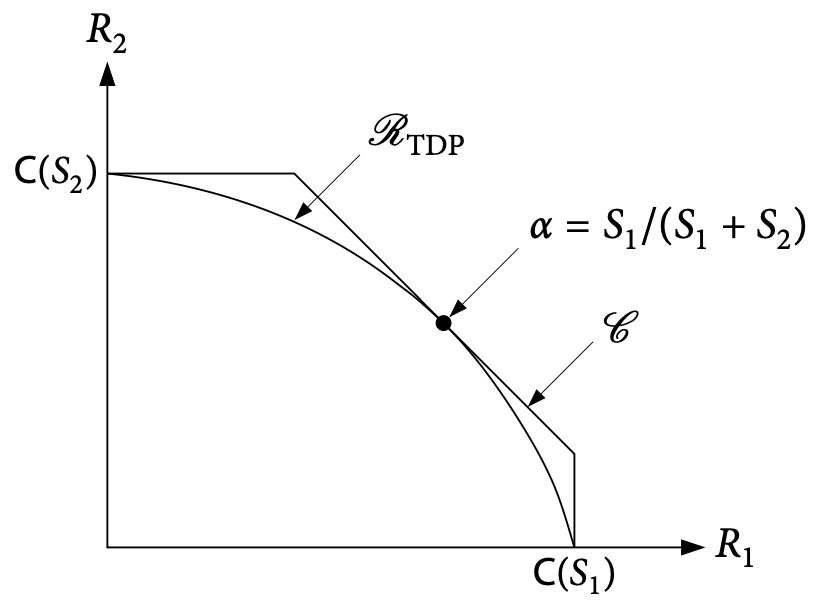
\includegraphics[width=0.9\textwidth]{figures/2tGMAC_pc.png}
            % \caption{ \Small TDP (time division with power control)}
        \end{figure}
    \end{column}
    
    \end{columns}

    \vfill

    \small The corner points of the Gaussian MAC capacity region can be achieved using \textcolor{red}{successive cancellation decoding}.         
    \end{frame}



    \begin{frame}[t]{Broadcast Channel, Downlink \small (1 sender, $K\geq2$ receivers)}
        \vspace{-1em}
        \begin{columns}
            % Column 2    
            \begin{column}{0.4\textwidth}
                \begin{figure}
                \centering
                    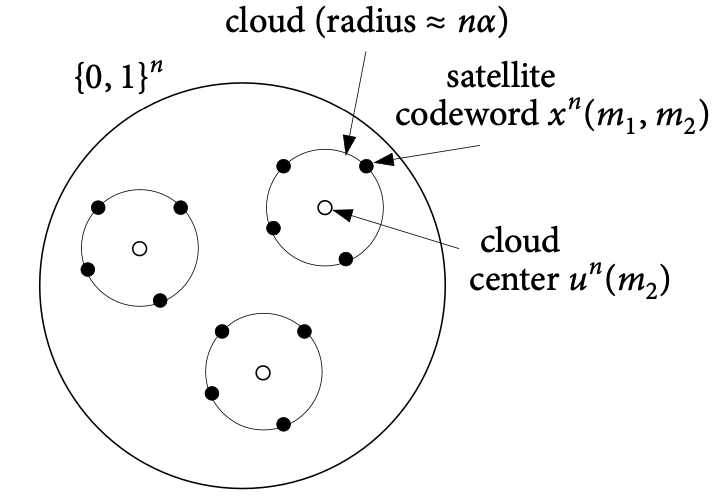
\includegraphics[width=0.9\textwidth]{figures/superpositioncoding.png}
                    % \caption{A figure that is next to a certain explanation.}
                \end{figure}
            \end{column}
    
            % Column 1
            \begin{column}{0.6\textwidth}
                \small
                \begin{theorem}[2Rx Superposition Coding Inner Bound]
                    If $\exists$ some pmf $p(u,x)$ such that rate pairs $(R_1,R_2)\in \mathbb{R}_+^2$ satisfying 
                    $$R_1 < I(X;Y_1|U),~ R_2 < I(U;Y_2),~ R_1+ R_2<I(X;Y_1).$$ Then $(R_1,R_2)$ is achievable. 
                \end{theorem}
            \end{column}
        \end{columns}

        \vfill
        
        In general, we do not know the capacity of BC. 
        
        However, superposition coding scheme attains capacity for \textcolor{red}{some} BCs. In particular, Gaussian BC is of a class called "degraded broadcast channels", whose capacity is known to be achieved by superposition coding. 
        
        \vspace{-0.3em}
        \begin{block}{Types of (discrete memoryless) Broadcast Channels}
            $$\underbrace{\text{Degraded}}_{\small \text{SC: capacity}} 
            \subsetneq \underbrace{\text{Less Noisy}}_{ \substack{\text{2,3Rx: SC is capacity} \\ \text{believe true for $\geq$ 4Rx} } }
            \subsetneq \underbrace{\text{More Capable}}_{ \substack{\text{2Rx: SC is capacity (El Gamal, 1978)} \\ \text{$3$Rx: SC strictly suboptimal (Xia \& Nair, 2012)} } }
            \subset \underbrace{...}_{\text{know little}} $$
        \end{block}
    \end{frame}

    \begin{frame}{Gaussian BC}
        \vspace{-1em}
        \begin{columns}
            % Column 2    
            \begin{column}{0.25\textwidth}
                \begin{figure}
                \centering
                    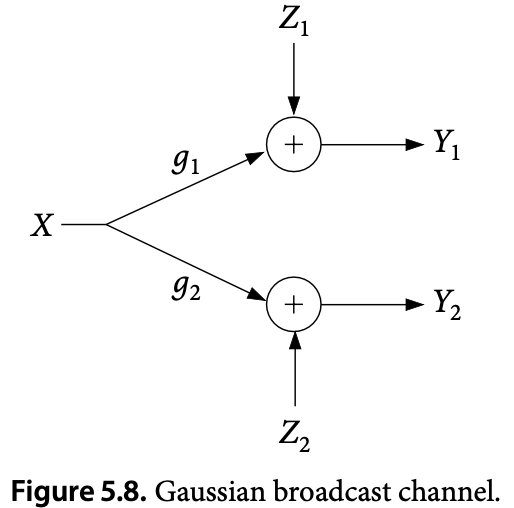
\includegraphics[width=0.9\textwidth]{figures/GBC1.png}
                    % \caption{A figure that is next to a certain explanation.}
                \end{figure}
            \end{column}
    
            % Column 2    
            \begin{column}{0.5\textwidth}
                \begin{figure}
                \centering
                    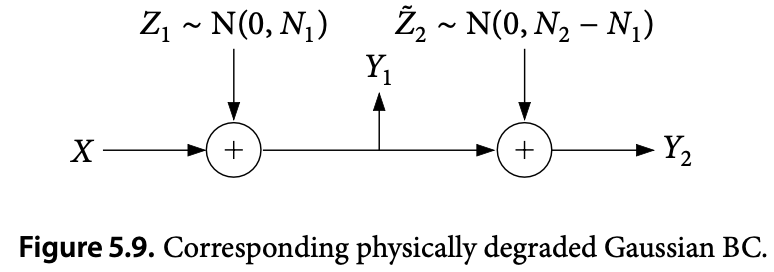
\includegraphics[width=0.9\textwidth]{figures/GBC2.png}
                    % \caption{A figure that is next to a certain explanation.}
                \end{figure}
            \end{column}
        \end{columns}

        \small 
        \begin{theorem}[Capacity region of 2Rx Gaussian BC $=$ SC-SIC ]
            The capacity region of Gaussian BC above is the set of rate pairs $(R_1,R_2)$ such that 
            $R_1 \leq \mathcal{C}(\alpha S_1), ~~R_2\leq \mathcal{C}(\frac{(1-\alpha)S_2}{\alpha S_1 + 1}),$ for some $\alpha \in [0,1]$, where $\mathcal{C}(x)$ is the Gaussian capacity function. $S_i$ denotes the signal-to-noise ratio of user $i.$
        \end{theorem}

        \vspace{-0.8em}
        \begin{theorem}[Capacity region of $K\geq2$-users Gaussian BC $=$ SC-SIC]
            The capacity region of $K$-user Gaussian BC is the set of rate pairs $(R_1,...,R_K)$ such that 
            $$R_k \leq \mathcal{C}(\frac{\beta_k S_k}{1+\sum_{j=1}^{k-1}\beta_j \gamma_k}),$$ for some $\alpha \in [0,1]$, where $\mathcal{C}(x)$ is the Gaussian capacity function.
        \end{theorem}

        
    \end{frame}

    
    \begin{frame}{OMA vs. NOMA in Gaussian MAC and Gaussian BC}
        \vspace{-0.3em}
        \begin{figure}
            \centering
                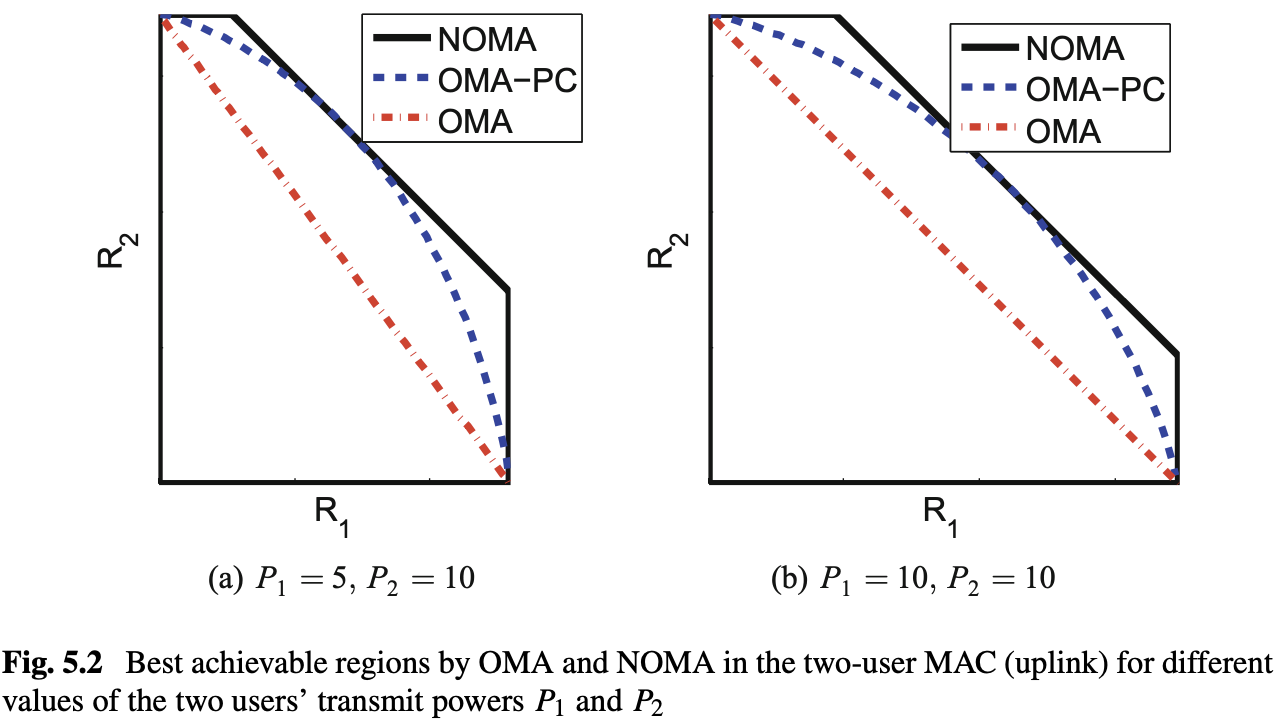
\includegraphics[width=0.53\textwidth]{figures/2tGMAC_vs.png}
                % \caption{A figure that is next to a certain explanation.}
        \end{figure}

        \pause
        \vspace{-0.3em}
        \begin{figure}
            \centering
                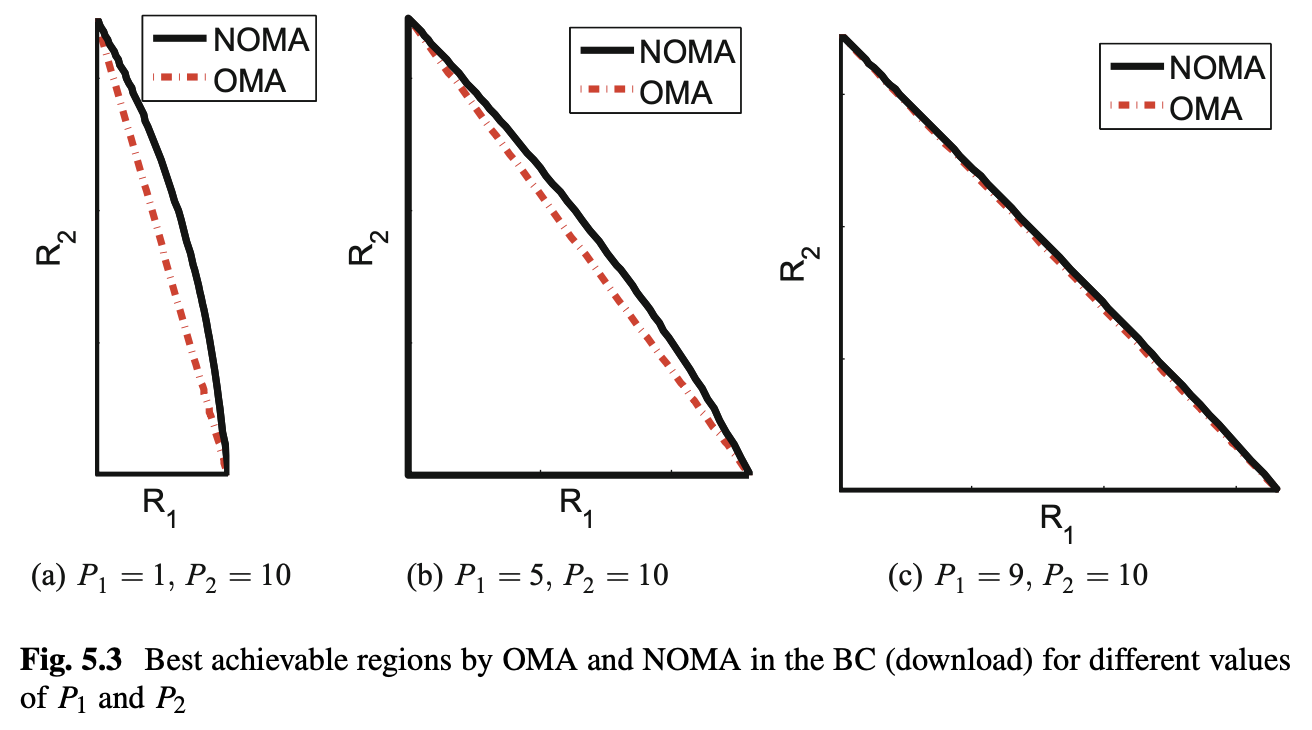
\includegraphics[width=0.59\textwidth]{figures/2rGBC_vs.png}
                % \caption{A figure that is next to a certain explanation.}
        \end{figure}
    \end{frame}


\section{NOMA in multi-cell: interference channel}
    \begin{frame}{Interference Channel \small ($\geq2$ senders, $\geq 2$ receivers)}
        Unlike previous MAC and BC, we really know little about interference channel, even for 2Tx-2Rx setting the capacity is unknown. Hence we focus on 2Tx-2Rx. 

        \vfill
        Even for Gaussian 2Tx-2Rx IC, capacity not known in general. 

        \begin{figure}
            \centering
                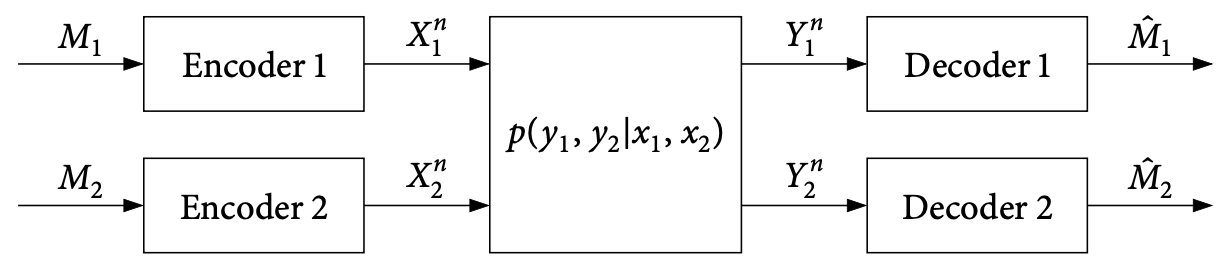
\includegraphics[width=0.73\textwidth]{figures/2t2rIC.png}
                \caption{Two sender–receiver pair DM-IC.}
        \end{figure}
        
        % In interference channels (aka, realistic channels) impose interference. However, recall that OMA schemes try to avoid interference! It turns out they need to spend huge price (far away from capacity) in IC. 
        \vfill
        Recall our theme: different schemes are... \textcolor{red}{all about dealing interference}. Let's see some examples now.
    \end{frame}

    \begin{frame}{Some inner bounds and outer bounds}
        \vspace{-1em}
        \small
        \begin{block}{Fix interference (individual capacity outer bound)}
            Maximal achievable individual rates are 
            $$R_1=C_1\leq \max_{p(x_1),x_2}I(X_1;Y_1|X_2=x_2), R_2=C_2\leq \max_{p(x_2),x_1}I(X_2;Y_2|X_2=x_1).$$
        \end{block}

        \vspace{-1em}
        \begin{block}{Avoid interference (time-sharing OMA inner bound)}
            $\forall \omega \in[0,1]$, $R_1 \leq \omega C_1$ and $R_2 \leq (1-\omega) C_2$. 
        \end{block}

        \vspace{-1em}
        \begin{block}{Compound MAC inner bound "Decode all". \textcolor{red}{Capacity for strong IC}}
            $\forall Q $ with $p(q,x_1,x_2) = p(q)p(x_1|q)p(x_2|q)$ satisfying 
            $$R_1 \leq I(X_1,X_2;Y_1|,Q), ~~R_2 \leq I(X_1,X_2;Y_2|Q), $$
            $$R_1 + R_2 \leq \min\{ I(X_1,X_2;Y_1|Q), I(X_1,X_2;Y_2|Q)  \}$$
        \end{block}
                
        \vspace{-0.5em}
        \begin{block}{Suffer interference (TIN IB) "Decode none": \textcolor{red}{Conjectured capacity for (very) weak IC}}
            $\forall Q $ with $p(q,x_1,x_2) = p(q)p(x_1|q)p(x_2|q)$ satisfying 
            $$R_1 \leq I(X_1;Y_1|Q), ~~R_2 \leq I(X_2;Y_2|Q). $$ 
        \end{block}
    \end{frame}

    \begin{frame}{Han-Kobayashi Inner Bound (1981)}
        \vspace{-0.7em}
        \begin{figure}
            \centering
                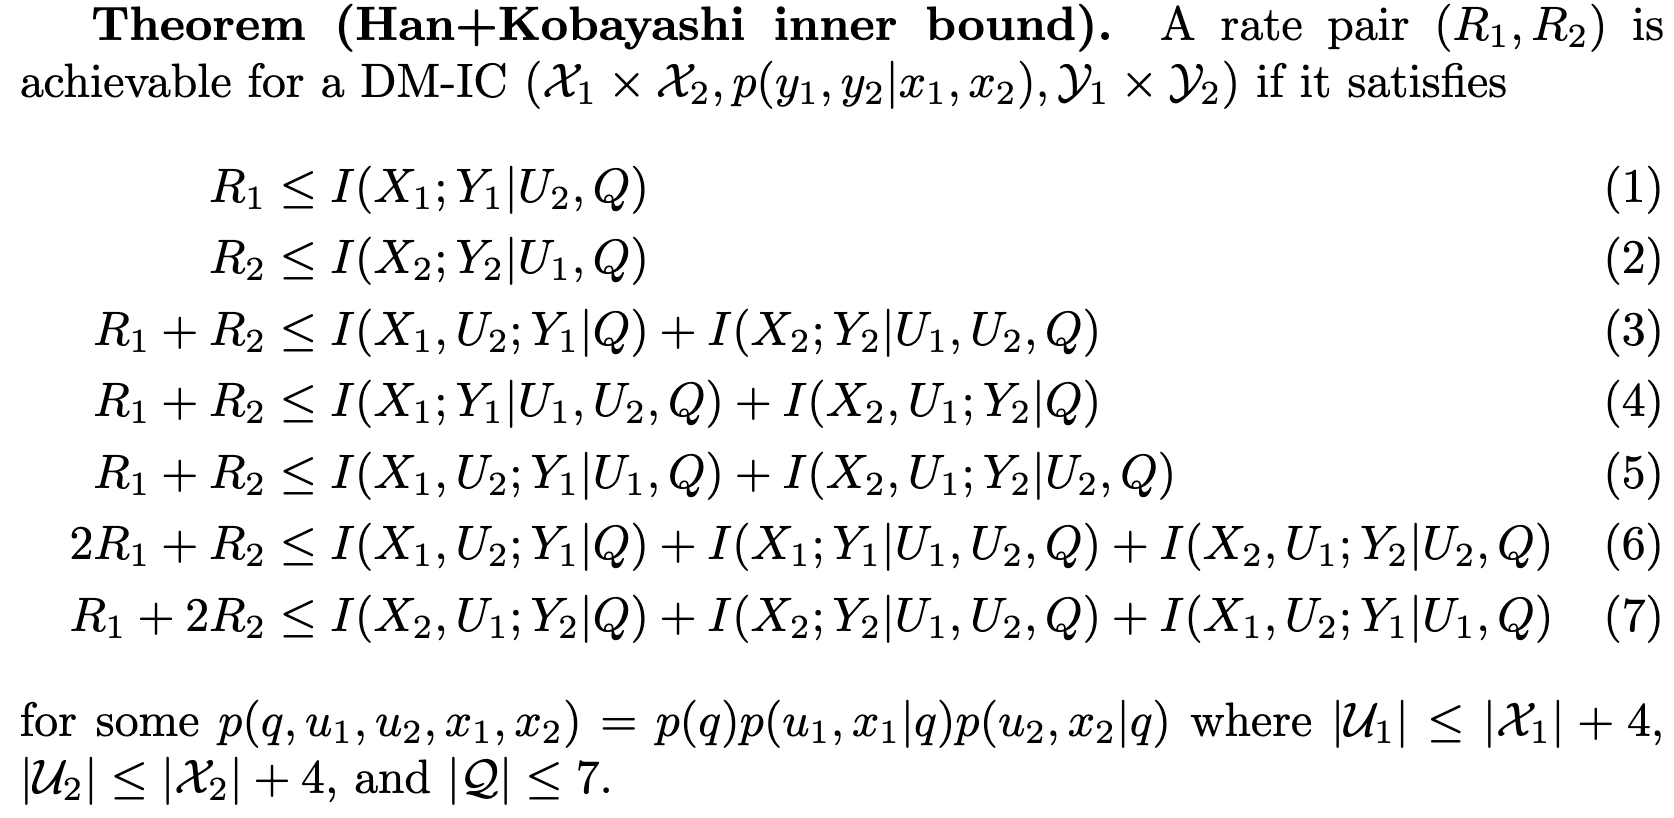
\includegraphics[width=0.6\textwidth]{figures/HKIB.png}
            \end{figure}

        \vspace{-1em}
        \small 
        \begin{remark}[HK inner bound: "decode some \& suffer the rest"]
            In the Han-Kobayashi (HK) scheme, each user split its message to be sent into two submessages of smaller rates and power. These are known as private and common messages. Common message is intended to be decoded only at the respective receiver, the private can be decoded at both receivers. 
            
            \textcolor{red}{The rationale behind this coding scheme is to decode part of the interference (the common message) and treat the rest as noise.}
        \end{remark}

        % \vspace{-0.7em}
         Examples show that HKIB cannot attain capacity in general. (Nair et al., 2015). 
         
         HKIB is only $\frac{1}{2}$ bit from capacity of 2Tx-2Rx Gaussian IC. (Etkin, Tse, Wang, 2008)
    \end{frame}

\section{Conclusion}
    \begin{frame}{Conclusion and Summary}
            Why we need NOMA now? Because we want to approach channel capacity promised by information theory.

            \vfill
            From theory's side, NOMA is the default mindset. Because as we saw, OMA schemes are (almost) always suboptimal, and we know this for decades. \textcolor{red}{From practice side, SC-SIC gives channel capacity for Gaussian MAC and Gaussian BC}.
             

            \vfill
            According to information theory, we know MAC the most, BC the second and we do not know much about IC. (\textcolor{red}{MAC, BC can be seen as a special case of IC}). 

            
            \vfill
            So, we would try NOMA schemes on MAC and BC first. This is indeed part of the focus of topics like machine-typed comm, massive connectivity, grant-free comm, etc.. 

            \vfill
            How to deal with interference from \textcolor{red}{another cell} in practice maybe not in the near future. If we do NOMA well enough intra-cell and just suffer interference from other cells, this will be aleady very good. 
    \end{frame}


\begin{frame}
  \begin{center}
  {\fontsize{40}{50}\selectfont Thank You!}
  \end{center}
\end{frame}

\begin{frame}{References}
    \small 
    M. Vaezi, Z. Ding, and H. V. Poor, Chapter 5 of "Multiple Access Techniques for 5G Wireless Networks and Beyond". Springer Publishing Company, Incorporated, 2018.

    \vfill 
    Natasha Devroye, “The interference channel”, \href{http://pfister.ee.duke.edu/nasit16/Devroye_slides.pdf}{online resource (slides)}, 2016

    \vfill 
    Abbas El Gamal and Young-Han Kim, “Network Information Theory” Cambridge University Press, USA, 2012.

    \vfill 
    L. Xia, Chapter 3, 4 of “On Tightness of Several Achievable Rate Regions in Network Information Theory”, 2016. 

    \vfill 
    Peng Xu, Zhiguo Ding, Xuchu Dai and H. Vincent Poor, "NOMA: An Information Theoretic Perspective", arXiv, 2015. 
    
\end{frame}



%***************************************************************************
%***************************************************************************
\end{document}





































